 %%LATEX header ********************************************
\documentclass[a4paper, 12pt, titlepage]{article}
\usepackage[utf8]{inputenc}
\usepackage[T1]{fontenc}
\usepackage[danish]{babel}
\usepackage{cite,refstyle,adjustbox,graphicx,amsmath,amssymb,subcaption,varioref,titlesec,comment,amsthm}
\usepackage{mathtools}
%\usepackage{epstopdf}
\usepackage{booktabs}
\usepackage{geometry}
\usepackage{setspace}
\usepackage{pgf,tikz}
\usepackage{fancyvrb}
\usepackage{parskip}
%%************************************************************
%%Teorem miljøer 
\newtheorem{antag}{Antagelse}
\newtheorem{teo}{Teorem}
%%************************************************************
%%Andet setup
\onehalfspacing
%%************************************************************
%% Makro
\newcommand{\indep}{\perp\!\!\!\perp}
\newcommand{\saa}{\Leftrightarrow}
\newcommand{\pd}[2]{\frac{\partial #1}{\partial #2}}
\newcommand{\Lagr}{\mathcal{L}}
%%************************************************************
%% Om forfatteren
%%************************************************************
\author{Simon Harmat og Niels Bækgård}
\title{Øvelse i produktivitetspolitik}
\date{\today}
\begin{document}
%\maketitle
%\tableofcontents
Hermed en analyse og vurdering af produktivitetsudfordringer særligt i Region sjælland

\section{Indledning}
Vi er interesserede i at undersøge, om der kunne være uudtømte effekt ved fra urbanisering i region Hovedstaden set i forhold til region Sjælland. 
\subsection{Motivation}
Der er store forskelle i timeproduktiviteten mellem region Sjælland og region Hovedstaden. En del af disse forskelle skyldes ganske givet branchesammensætning, hvor mere produktive brancher fylder mere i region Hovedstaden end de gør i region Sjælland. Men det kan ikke forklare det hele.

Hvis man i stedet sammenligner samme brancher og dermed ser på, hvad produktivitetsforskellen måtte være her, da vil det være muligt at udrede om der gives urbane produktivitetseffekter. Dette kalder vi for \emph{urban learning}.
\section{Teori}
\subsection{Agglomeration}

I dette afsnit vil vi gennemgå den økonomiske teori bag agglomeration og baggrunden for, hvorfor agglomeration påvirker produktivitet. Introduktionen til begrebet er primært baseret på bagrund af bogen \emph{"Econonmics of Agglomeration"} (2013) af Fujita og Thisse.

\subsection{Definitioner og introduktion}
Agglomerationsøkonomi betegner en positivt eskternalitet som opstår, når økonomiske personer eller virksomheder drager nytte af være fysisk tæt på hinanden. 

Agglomeration er indenfor den økonomiske litteratur et relativt nyt aspekt. Især har det været benyttet til at approksimere de brede eller eksterne økonomisek effekter af transportomkostninger, der tidligere ikke har været tilstrækkeligt inddraget i typiske cost-benefit analyser.

Motivationen for at inddrage agglomeration i sådanne analyser er, at investeringer i infrastruktur sænker den effektive distance mellem økonomiske agenter, hvilket både har interne og eksterne effekter. De interne effekter er fx mindre rejsetid, færre transportomkostninger, mens de eksterne effekter ved agglomeration er gennem videnskudveksling, større innovation, større specialisering. Relevansen for disse eksterne effekter i en vores sammenhæng er, at de medfører en forøgelse af produktiviteten.

Definitionen på agglomeration er angivet

Intuitionen bag denne er lang



\textbf{Et større og tættere arbejdsmarked} som betyder bedre matching mellem arbejdsudbuddet og virksomhedens efterspørgsel af arbejdskraft. Endvidere tillader et stor arbejdsmarked også mere specialisering af arbejdsudbuddet. Dette sker både fordi arbejdskraften har mulighed for at akkumulere human kapital, men også fordi arbejderne har mulighed for at drage nytte af hinandens human kapital.  

\textbf{Fælles brug af leverandører og infrastruktur.} Virksomheder kan drage nytte af flere om at efterspørge mellemvare eller infrastruktur som kræver store faste omkostninging. Dette kunne eksempelvis være en havn, hvor en stor efterspørgsel gør det muligør og rentabelt for en levendør  at foretage investering i nye, og mere effektive, terminaler. På samme måde kan producerenter mindske diversiteten af deres produktporteføljer, og dermed få produktivtetsforbedring gennem specialisering og skala økonomi.    

\textbf{Produktivitetforbedring gennem vidensdeling.} Spillover af viden kan ske under formelle og uformelle rammer. De formelle rammer kan dannes gennem fx konferrencer, forskningsnetværk, konsulenter eller samarbejde virksomheder imellem. De uformelle rammer sker gennem arbejdskraften. Arbejdskaften kan få ny viden mellem netværk, eller når medarbejdere skifter job, således at en ny virksomhed kan drage nytte af medarbejdernes viden og læring. \cite{sorensen2014infrastruktur}  


Effekterne ved agglomeration bliver ofte opdelt i to teoriske klasser: \emph{lokaliseringsøkonomi} og \emph{urbaniseringsøkonomi}. Lokaliseringsøkonomi er et begreb der bruges når koncentration af ensartet industrier er stor. Ensartet virksomheder som er placeret geografisk tæt på hinanden kan drage fordel af teknologiske fremskidt hos hinanden, således at en klynge af virksomheder specialiceres og dermed får en komparativfordel i særlige produktioner. Dette gør virksomhederne mere produktivte og kan forklare produktivitetsvækst i industrielle distriker.  Det andet begreb, urbaniseringsøkonomi, handler i højere grad om de positive effekter som opstår når virksomheder og arbejdskraften koncenterer sig geografisk, men begge karakteriseret som alsidige. Alsidigheden betyder at brancher kan drage nytte af hinandens teknologiske fremskridt, general markedsstørrelser og fælles infrastrukturen. Studier som beskæftiger sig med de to effekt seperat peger på, at effekterne ved lokaliseringsøkonomi typisk er størst, mens at videnstunge service virksomheder oplever positive effekter ved urbanisering \cite{melo2009meta}. I denne opgave vil vi ikke skelne mellem disse to typer for agglomeration, men som et begreb der indeholde effekter både fra lokalisering og urbanisering.


Der kan dog også  opstår negative effekter ved agglomeration. 

Negative effekter ved agglomeration

Agglomeration kan også øges ved bedre infrastruktur for på den måde at mindske den fysiske afstand mellem byer og mennesker

lokaliseringsøkonomi og urbanisering, forskel mellem de to. Vores mål adskiller ikke de to. I meta-analysen skriver de at det ikke gør den store forksel overordnet


\subsection{Produktivitetskommissionen}
\subsection{Debatindlæg fra CE}
\section{Metode}
\subsection{Målning af agglomertaionseffekter med effektiv tæthed }

Der findes flere fremgangsmetode når agglomerationseffetker skal estimeres. Fælles for metoderne er at danne et mål som skal repræsentere skala af økonomiske aktivitet i en geografisk kontekst,indgå som variable i estimationen af produktiviteten og dermed modellere eksternaliteten ved agglomeration. I meta-analysen \cite{melo2009meta} gennemgår forfattterne evolutionen af disse forskellige metoder. De tidligeste eksempler fokuserede udelukkende lokale byeffekt og berorede sig ofte på indbyggerantal. Problemet ved disse mål er, at indbyggerantal i et givent område ikke alene er et udtryk for den stedsbestemte økonomiske aktivitet, men indbyggerantallet vil også være et udtryk for bystørrelser.

Sidenhen blev beskæftigelsestætheden indtroduceret. Fordelen ved dette mål er at den lokale beskæftigelse mere isoleret udtrykker den økonomiske aktivitet, og derved er et bedre mål for produktivitetsfordele. Tæthedsaspektet gør også målet robust overfor størrelsesforskellige områder imellem. 

Fælles for begge mål er, at der implicit i målene er en antagelse om afgrænsede markeder, områder imellem. Dette betyder, at områdernes relative afstand ingen betydning har, og områderne kan ikke drage nytte af hinandensmarkedede, og derved opnå spillover effekter. Spillover effekter i form af større arbejdsmarkeder mht. matching, vidensdeling eller specialisering. For både at tage højde for skalaen af økonomisk aktivitet og nærheden af andre lokaløkonomier eller markeder udviklede nogle studier en anden metode.  

Dette ses blandt andet i studiet \cite{graham2007agglomeration}. Her introducere Graham en parameter, effektiv tæthed, som måler den økonomiske aktivitet i et område, ift. beskæftigelsestætheden, og områdets relative geografisk afstand til andre økonomiske områder ift. deres repsektive beskæftigelsestætheden . Med andre ord indfanger parameteren effekt ved den relative afstanden til andre potentielle markeder, således forsvinder den implicitte antagelse om afgrænsning områderme i mellem, og målet tillader en afsmittende effekt ved agglomeration. To nærliggende områder med høj beskæftigelsestæthed for altså lov til at drage fordel af hinanden, men effektive tæthed er aftagende i afstand. Parameterens formål er altså at indfange de samlede agglomerationseffekter, og skelner derfor ikke mellem lokaliserings- og urbaniseringsøkonomi. Hvor fordele ved lokaliseringsøkonomi tilsiger vidensspillover gennem em koncentration af ensartet industri. Mens fordelene ved urbaniseringsøkonomi baserer sig på vidensspillover gennem diversitet og massen af forskellighed. Selv om dette selvfølgelig kan være interessant, så fastslår Graham at dette ikke har den store effekt når man ønsker at estimere den samlede eksternaliteten ved agglomeration med henvisning til et tidligere studie lavet af Graham selv.


 %%%Figur
\begin{figure}[h!]
    \centering
    \begin{subfigure}[b]{0.49\textwidth}
        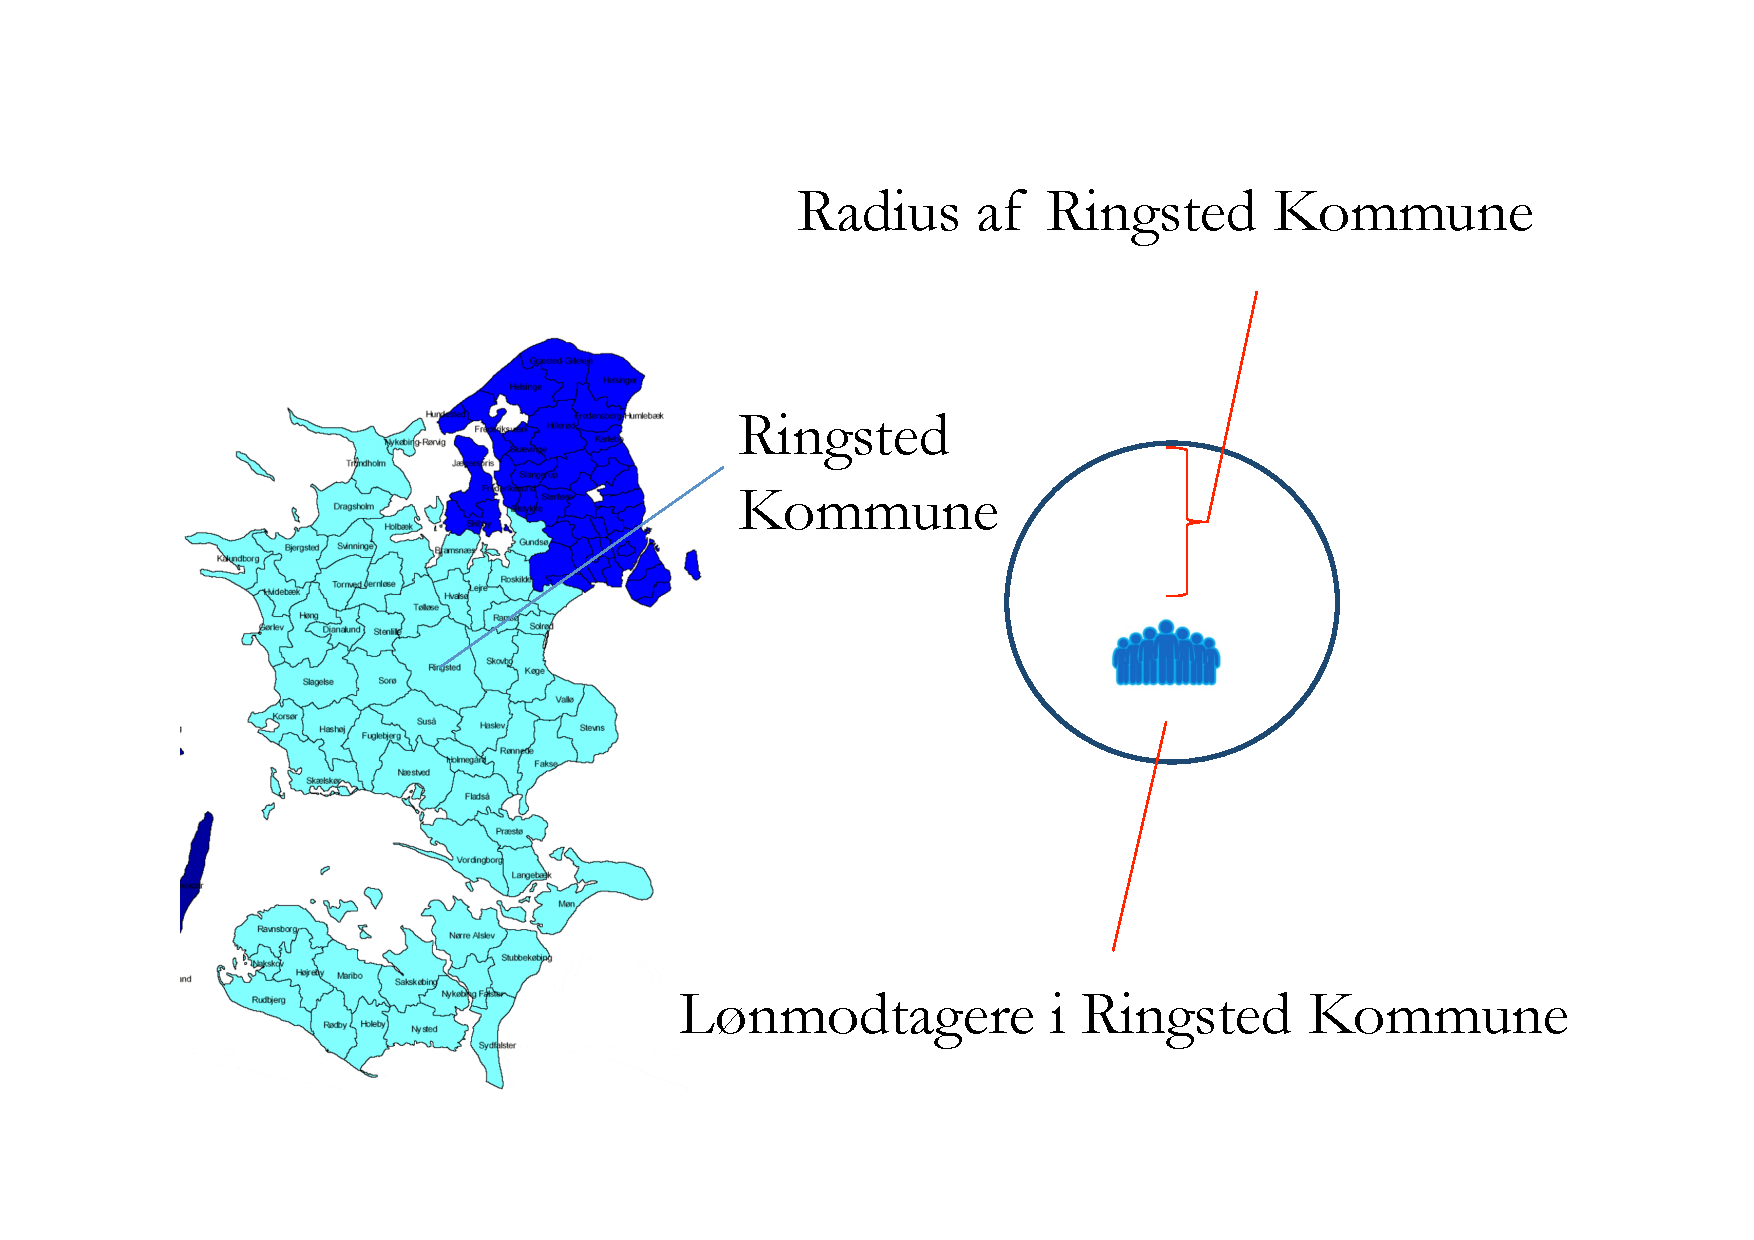
\includegraphics[width=\textwidth]{del1.pdf}
        \caption{Beskæftigelsestætheden}
        \label{fig:del1}
    \end{subfigure}
    \begin{subfigure}[b]{0.49\textwidth}
        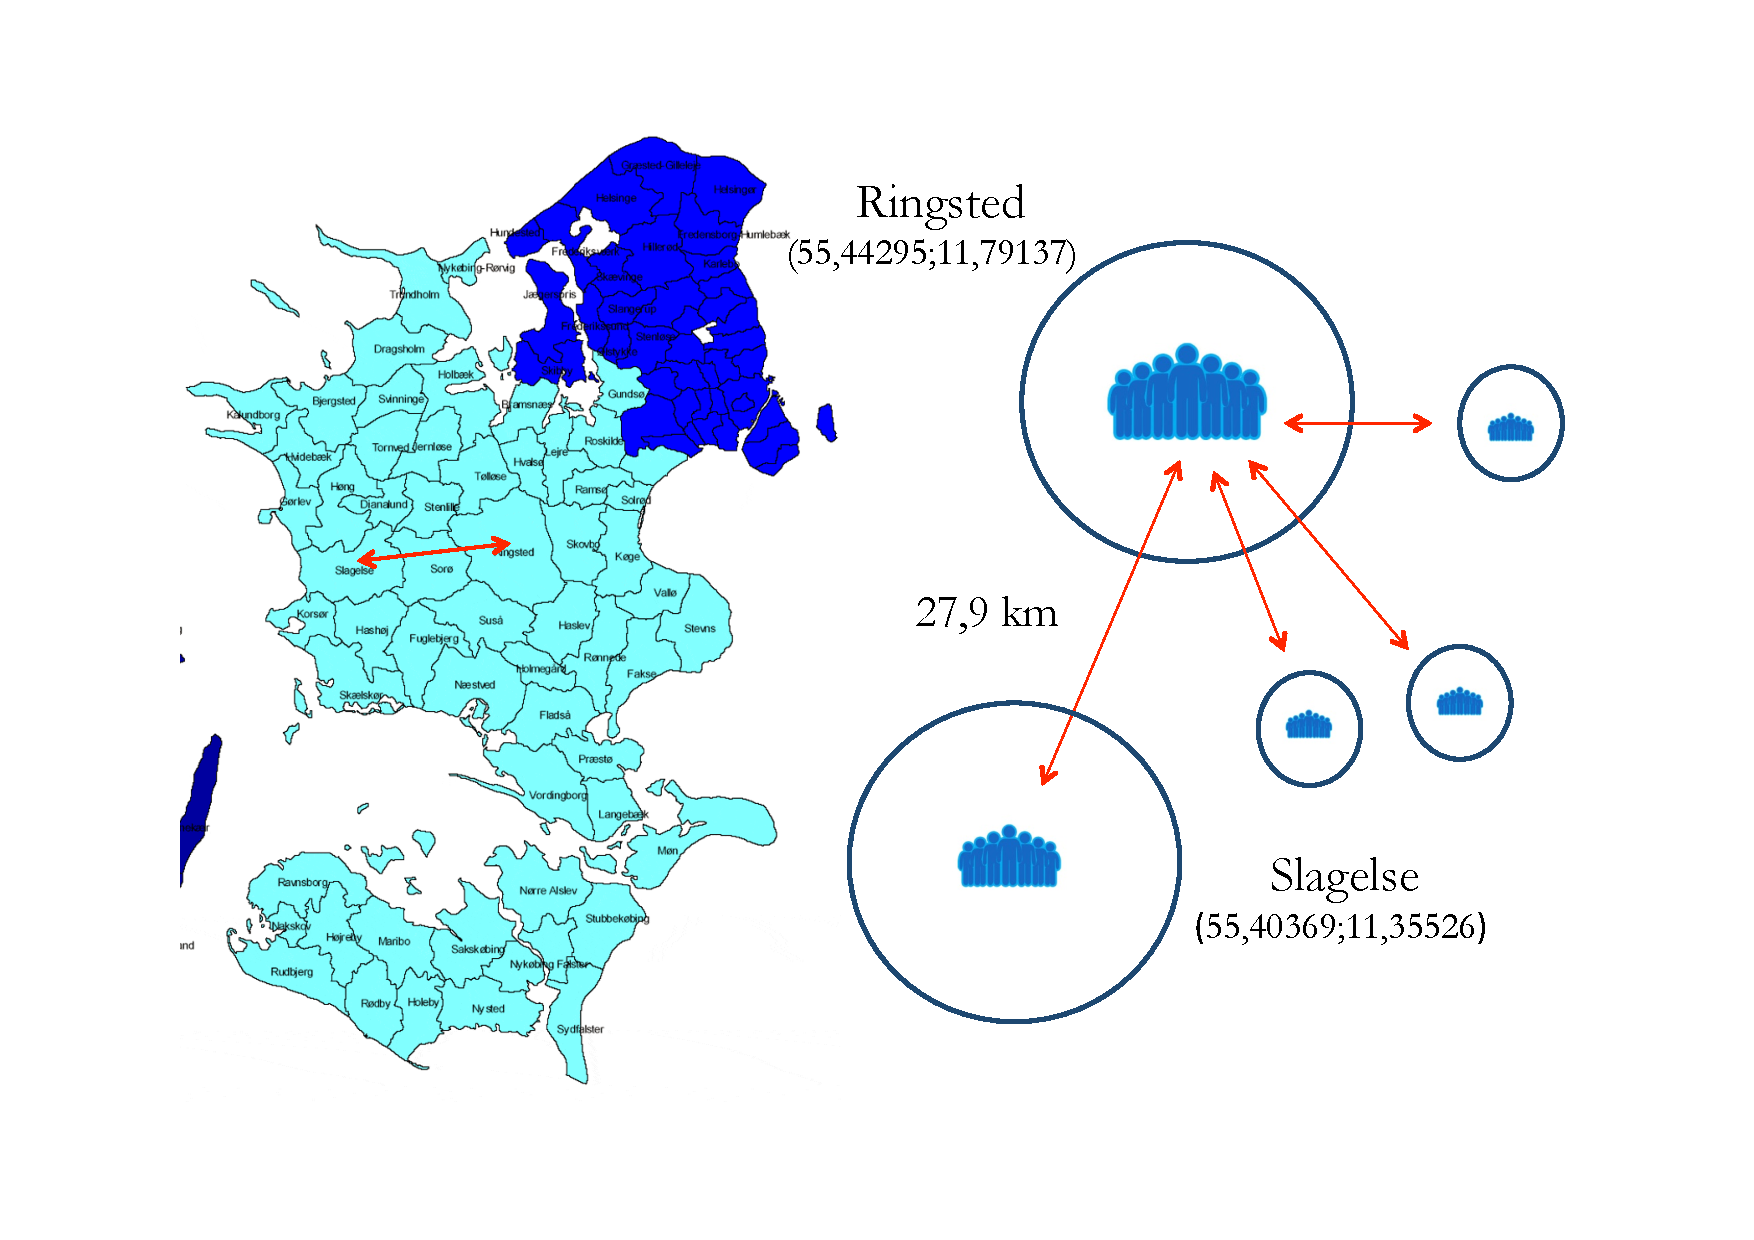
\includegraphics[width=\textwidth]{del2.pdf}
        \caption{Potentielle marked}
        \label{fig:del2}
    \end{subfigure}
  \caption{Caption here}
  \label{fig:metode}
\end{figure}




Til vores analyse har vi valgt, at konstrure parameteren effektiv tæthed, $ED$, i tråd med Grahams metode jf.\cite{graham2007agglomeration}. Fremgangsmetoden kan med fordel forklares med et eksempel som illusteret i figur \ref{fig:metode}. Vi tager de enkelte kommuner, her Ringsted Kommune, og benytter antal af registerbaseret beskæftigelse efter arbejdssted\footnote{Registerbaseret arbejdsstyrke, beskæftigelse, tabel RAS301, Danmarks Statistik} til skalaen af den økonomiske aktivitet. For at udregne tætheden af beskæftigelsen i Ringsted Kommune, finder vi forholdet mellem beskæftigelsen i kommunen og kommunensstørrelse målt på radius kilometer, det betyder at vi implicit antager at kommunerne er cirkelformet. Når vi kender arealet på kommunerne, kan vi blot udregne radius ved hjælp af formlen for radiusen af en cirkel. Denne antagelse viser sig nyttig, når vi skal udregne den relative anstand kommunerne og deres økonomiske aktivitet i mellem. Derefter skal vi bestemmer midtpunkten alle kommunerne, for så at udregne beskæftigelsen per afstandskilometer til alle de 97 andre kommuners midtpunkt. 

$ED$ måler altså den agglomeration som hver virksomhed oplever givet deres placering i Danmark. Første led er selve agglomerationen i hjemkommunenen, $j$, mens andet led er den agglomerationseffekt virksomhederne oplever fra resten af landets kommuner som er faldende i aftand. Virksomhederne i Ringsted Kommune påvirkets altså positivt af en høj beskæftigelse i hjemmekommune, samtidigt påvirkets virksomhederne relativt mere af en høj beskæftigelse i nærliggende kommuner, såsom Slagelse, forhold til jyske kommuner. En væsenligt afgrænsning i vores mål er, at vi ikke tilader agglomerationeffekter på tværs er landegrænser. Det betyder at byer som Flensborg og Malmø ikke indgår i analysen, men pendlerne som rejser på tværs af landene for at arbejde indgår i bæskiftigelsen. Hvis agglomerationseffekter skal indgå i evalueringen af national politik initiativer er tabet ved denne forsimpling ikke stor - hvis derimod fordelen ved en Øresundsbro eller Fermenforbindelse skal evalueres kan analysen med fordel udvides. Den effektive tæthed kan opskrives på følgende vis: 

\begin{equation}
   ED^j_t = \frac{L^j_t}{Radius_j} + \sum_{k=1}^{k \neq j} \frac{L^k_t}{d_{kj}}, \quad Radius_j = \sqrt{\frac{A_j}{\pi}}
 \end{equation} 
 hvor $d_{kj}$ er afstanden mellem kommune $k$ og $j$. 
 

For at finde afstandene mellem alle 98 kommuner i Danmark, benytter vi en såkaldt API. En API gør det muligt at automatisere forspørgelser til en server, i dette tilfælde til servicen Google Maps gennem programmet \textsf{R}. Ved at sende navnet på kommune returnere Google Maps en lokalation i form af koordinat i breddegrader og længdegrader. Vi antager at denne lokation er det approksimative økononomiske midtpunkt af en given kommune. 

Dernæst udregner vi afstanden mellem to kommuners koordinater vha. Haversine-formel\footnote{Skriv en lille historie}. Haversine-formel beregner den korteste afstanden mellem to punkter på en sfære, hvilket netop giver fulgefulgt mellem to kommnuernes midtpunkter. Således kan vi udregne afstandende på kryds og tvær af alle kommuner i en $98\times 98$ symmetrisk matrice. Her er det vigtigt at pointere, at vores afstandsmål ikke tager hensyn til den faktiske kørselsafstand mellem to kommuner. Dette betyder at tolkning af parameteren er den procentvise produktivitetsgevinsten hvis afstanden mellem virksomheder/arbejdskraften mindske med en procent. 

Vi udregner $ED$ for perioden 2008-2015\footnote{En oversigt over effektiv tæthed i perioden 2008-2015 for alle 98 kommuner findes i Appendix}. Hvis vi betragte gennemsnittet af variablen i løbet af perioden, ser vi at de kommuner som er placeret i hovedstadsområdet har den højste værdi. Dette skyldes den høje tæthed af beskæftigelse i København og Frederiksberg. Frederiksberg, Rødovre og København har de tre højste værdi, efterfulgt af de andre kommuner i Storkøbenhavn. Yderligere se vi nogle af de større midtsjællandske kommuner også drager fordel af deres relative afstand til hovedstadsområdet. Aarhus er placeret som nummer 32, efterfulgt af nogle nabokommuner såsom Skanderborg og Odder. Fyns og midtjyllands kommuner findes midt på listen. Den lave ende af listen er kendetegnet ved kommuner, vis placering ofte betegnes som værende i den rådne banan. Det er kommuner som er placeret tæt på den jyske vestkyst. Dette er kommuner såsom Frederikshavn, Hjørring Thisted og Lemvig. I bunden af listen finder vi Bornholm og Læsø som 'staffes' for både at have en tynd besæftigelsestæthed og deres geografiske placering.

Hvis vi betragter ændringen i effektiv tæthed fra 2008 og 2015 tegner der sig en klart billed af urbanisering omkring hovedstaden. Dette er illusret på Danmarkskortet i figur \ref{fig:aendring}. Region Hovedstaden er som en den eneste region, hvor den effektive tæthed har udviklet sig positivt. Aarhus og de omkringliggende kommuner er næsten uændret i perioden, altså neutral eller svag mindskning af effektiv tæthed. De kommuner hvor udviklingen har været mest negativ på tværs af den 'rådne banan', atlså Midt og Vestjylland, Sønderjylland,Fyn og Sydsjælland.

\begin{figure}[tb] 
  \centering
  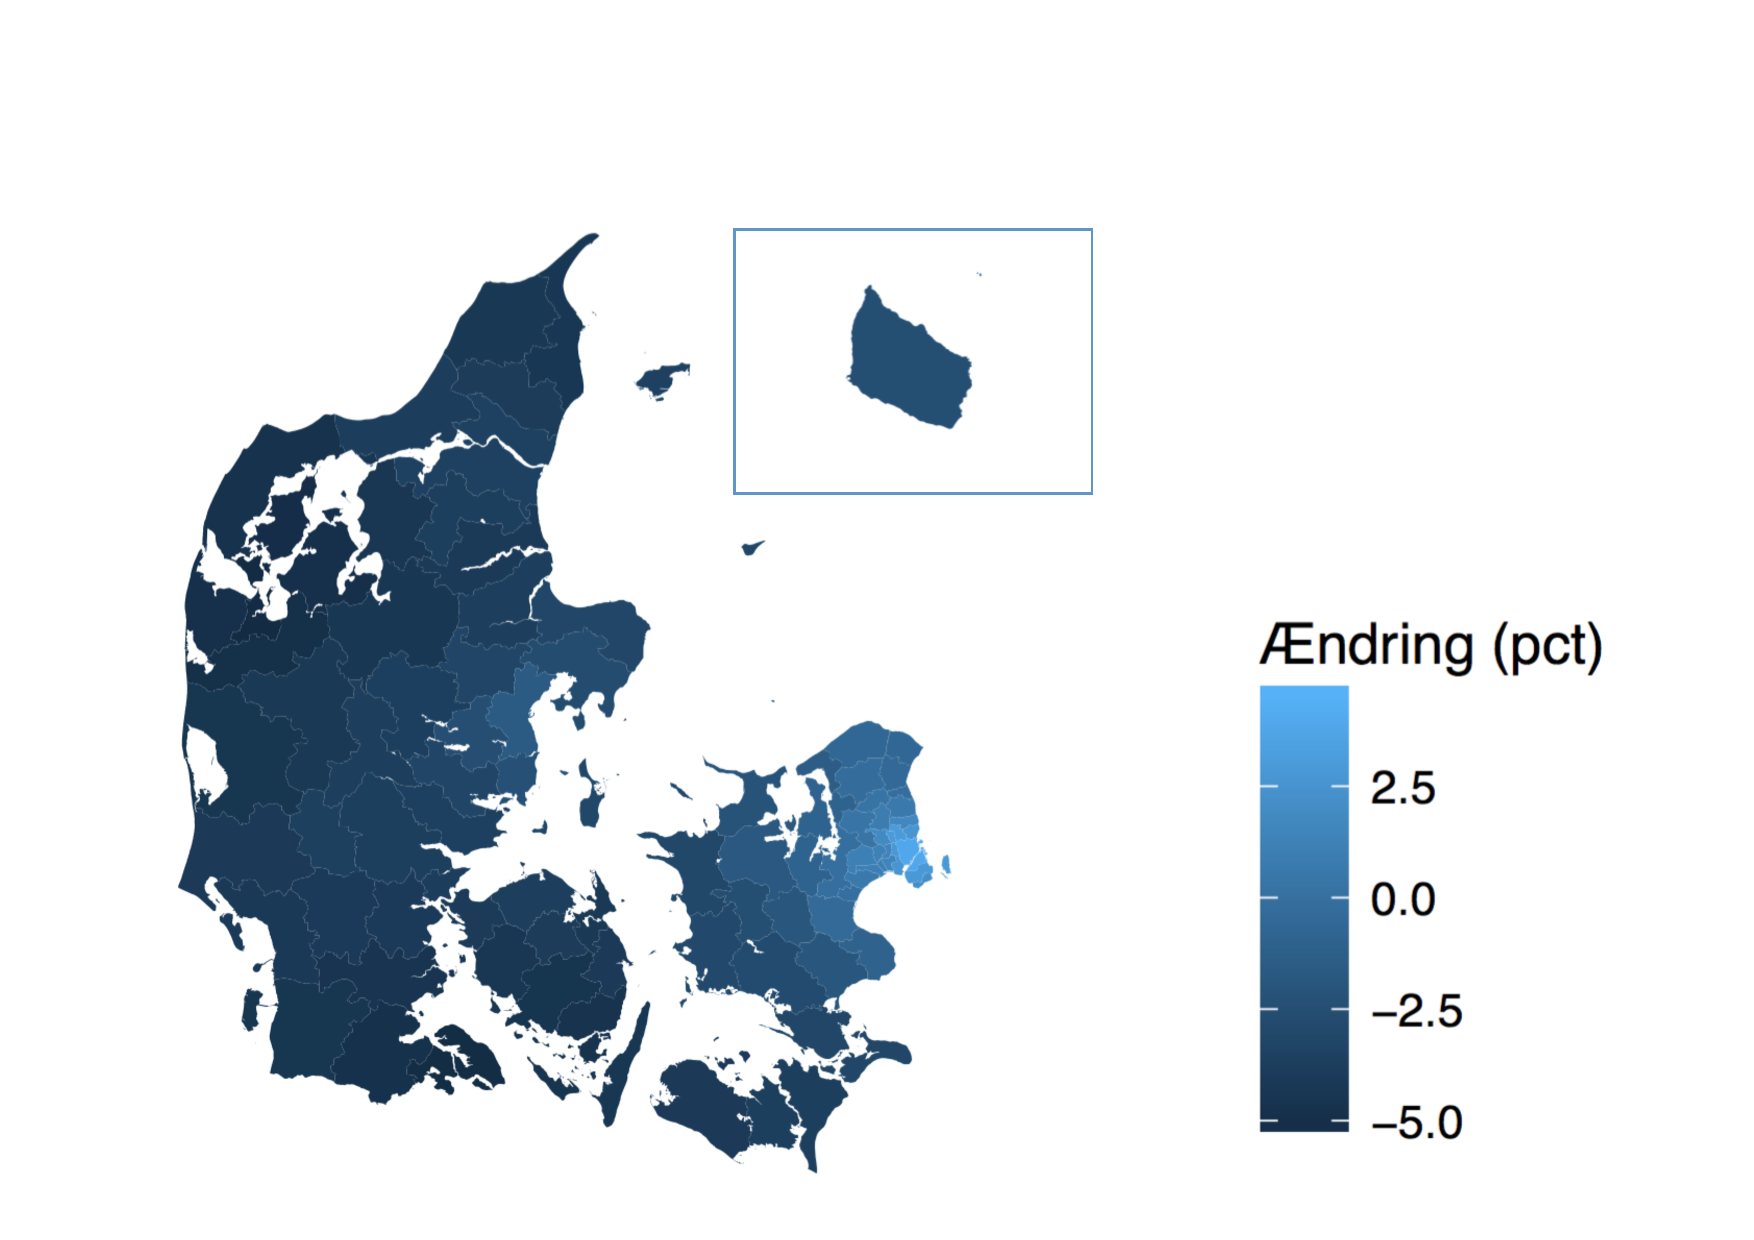
\includegraphics[width=\textwidth]{andring.pdf}
  \caption{Ændring i effektiv tæthed i Danmark 2008-2015, pct.}
  \label{fig:aendring}
\end{figure}

  
  
  Skrald
  Opgørelse af dette For at medtage intensiteten på tværs af kommunerne, sætter vi antal beskæftigede i forhold til arealet af kommunerne. Fordelen ved at benytte beskæftigelsestæthed istedet for indbyggertætheden er: 1) antal beskæftigede fanger bedre produktivitetsfordelen ved geografiske konsentreret økonomisk aktivitet, mens at indbygger også vil agere som proxy for urbanisering og eventuelle traffik omkostninger. Ved at benytte tætheden, altså antal eskæftigede lønmodtagere forhold til areal, gør målet robust overfor forskellige kommune størrelser \cite[pp. 335.]{melo2009meta}.
 
men tager ikke højde for l. Forskellen på lokaliseringsøkonomi og ur
Graham har estimeret forskellige effekter ved urbanisering vs. clusters i et andet papir (Graham 2006)  
 Lokaliseringsøkonomi
• Vidensspillovers baseret på ensartet produktion
– Klynger, ældre industrier – Urbaniseringsøkonomi
• Videsspillovers baseret på diversitet
– Massen af forskellighed, nyere industrier



..


 
 


\section{Data}
\section{Estimation}
Vi ønsker at estimere følgende output dataset
\begin{equation}
	\ln Y_{it}^{pj} = \alpha^p_0 + \ln K_{it} + \ln L_{it} + ED^j_{t} + \omega^p_{t}
\end{equation}
hvor $i$ er virksomhedsindeks, $p$ kommuneindeks, $t$ angiver tidspunkt i år og $j$ angiver kommune. 
\section{Praktisk case/vinkel}
\section{Diskussion}
Forslag: Kvalitetsjustering af beskæftigelsen i ED og lag værdier af ED 
\section{Konklusion}



\paragraph{Kvalitetsjusteret arbejdskraft}



\paragraph{Levihnson og Petrin}
Hvad nu hvis jeg skriver noge

Syntaksen for at citere er \cite[pp. 211ff.]{melo2009meta}. 

 % paragraph levihnson_og_petring (end)



\bibliography{prodBib.bib}
\bibliographystyle{plain}
\end{document}